\subsection{Restaurant use cases}

\noindent \textbf{x. Use case: Create a new menu}
\begin{center}
  \begin{tabular}{| l | p{10.75cm} | }
    \hline
    Actor        & Restaurant \\
    \hline
    Scenario     &
    \begin{minipage}[t]{\linewidth}
      \begin{enumerate}[leftmargin=*,nosep,before=\vspace{-0.575\baselineskip},after=\strut]
        \item The restaurant employee presses a button for creating a new menu.
        \item The application displays a screen with an empty menu. \textbf{A1} \textbf{A2} 
        \item The restaurant employee specifies meta-information about the menu. \textbf{A3}
        \item The restaurant employee specifies the restaurant's contact information. \textbf{A4} \textbf{A5} 
        \todo[inline]{Extension point - all menu options}
        \item The restaurant employee specifies when shall the menu be valid. (Extension point)
        \todo[inline]{Extension point - Warn my guests about allergens in the foods I serve}
        \item The restaurant employee specifies how shall the menu display allergen information. (Extension point) 
        \item The restaurant employee adds categories to the~menu.~\textbf{A6}
        \item The restaurant employee adds individual food items to the menu.
        \item The restaurant employee presses a button for saving the menu.
        \todo[inline]{Extension point - publish, print}
        \item The application saves the menu. \textbf{A7} (Extension point)
      \end{enumerate}
    \end{minipage}
    \\
    \hline
    Alternatives &
    \begin{minipage}[t]{\linewidth}
      \begin{description}[nosep,after=\strut]
        \item [A1:] The restaurant employee selects that they wish to use a template. The application displays a menu with some predefined content.
        \item [A2:] The restaurant employee selects that they wish to create the menu based on an existing menu. The application displays a menu with the contents of the base menu.
        \item [A3:] Meta-information is loaded from the restaurant's profile and inserted to the menu by the application.
        \item [A4:] The restaurant employee does not wish to include the restaurant's contact information in the menu and skips this process. 
        \item [A5:] The application inserts the restaurant's contact information automatically based on the restaurant's profile.
        \item [A6:] The restaurant employee skips the creation of categories.
        \item [A7:] The restaurant employee forgets to specify one of the menu's meta-information options. The application warns the restaurant employee about this fact. The restaurant employee finalizes the creation of the menu and the scenario continues with step 9.
      \end{description}
    \end{minipage}
    \\
    \hline
  \end{tabular}
  \newline
\end{center}

\newpage

\noindent \textbf{x. Use case: Warn my guests about allergens in the foods I serve}
\todo[inline]{add use case number in extends column}
\begin{center}
  \begin{tabular}{| l | p{10.75cm} | }
    \hline
    Actor        & Restaurant \\
    \hline
    Description        & A restaurant employee wants to add information about allergens contained in a menu's items. \\
    \hline
    Extends       &  x: Create a new menu \\
    \hline
    Scenario     &
    \begin{minipage}[t]{\linewidth}
      \begin{enumerate}[leftmargin=*,nosep,before=\vspace{-0.575\baselineskip},after=\strut]
        \item The restaurant employee specifies that numbers shall be used to indicate allergens contained in menu items. \textbf{A1}
        \item The application inserts a predefined allergen table at the end of the menu.
        \item The application later automatically inserts allergens to menu items based on their ingredients.
      \end{enumerate}
    \end{minipage}
    \\
    \hline
    Alternatives &
    \begin{minipage}[t]{\linewidth}
      \begin{description}[nosep,after=\strut]
        \item [A1:] The restaurant employee specifies that allergen labels shall be used in the menu. The scenario continues with step 3.
      \end{description}
    \end{minipage}
    \\
    \hline
  \end{tabular}
  \newline
\end{center}

\noindent \textbf{x. Use case: Create a stable menu}
\begin{center}
  \begin{tabular}{| l | p{10.75cm} | }
    \hline
    Actor        & Restaurant \\
    \hline
    Description  & A restaurant's management wants its restaurant to have a stable menu which will be valid every day of the week. \\
    \hline
    Extends       &  x: Create a new menu \\
    \hline
    Scenario     &
    \begin{minipage}[t]{\linewidth}
      \begin{enumerate}[leftmargin=*,nosep,before=\vspace{-0.575\baselineskip},after=\strut]
        \item The restaurant employee selects that the menu shall be valid every day of the week. \textbf{A1} 
        \item The restaurant employee chooses an option that the menu shall repeat periodically for the selected days.
        \item The restaurant employee specifies that the menu shall be valid all day.
      \end{enumerate}
    \end{minipage}
    \\
    \hline
    Alternatives &
    \begin{minipage}[t]{\linewidth}
      \begin{description}[nosep,after=\strut]
        \item [A1:] The restaurant employee selects the option that the menu will be a stable offer menu. The application inserts the information about what days of the week shall the menu be valid and when automatically.
      \end{description}
    \end{minipage}
    \\
    \hline
  \end{tabular}
  \newline
\end{center}

\noindent \textbf{x. Use case: Create a stable menu in a foreign language}
\begin{center}
  \begin{tabular}{| l | p{10.75cm} | }
    \hline
    Actor        & Restaurant \\
    \hline
    Description  & A restaurant's management wants its restaurant to have a stable offer menu written in a foreign language. \\
    \hline
    Extends       &  x: Create a new menu \\
    \hline
    Scenario     &
    \begin{minipage}[t]{\linewidth}
      \begin{enumerate}[leftmargin=*,nosep,before=\vspace{-0.575\baselineskip},after=\strut]
        \item The restaurant employee selects that the menu shall be valid every day of the week. \textbf{A1}
        \item The restaurant employee chooses an option that the menu shall repeat periodically for the selected days.
        \item The restaurant employee specifies that the menu shall be valid all day.
        \item The restaurant employee later adds categories and menu items in the desired language.
      \end{enumerate}
    \end{minipage}
    \\
    \hline
    Alternatives &
    \begin{minipage}[t]{\linewidth}
      \begin{description}[nosep,after=\strut]
        \item [A1:] The restaurant employee selects the option that the menu will be a stable menu. The application inserts the information about what days of the week shall the menu be valid and when automatically. The restaurant employee continues with step 4.
      \end{description}
    \end{minipage}
    \\
    \hline
  \end{tabular}
  \newline
\end{center}

\noindent \textbf{x. Use case: Create a list of beverages}
\begin{center}
  \begin{tabular}{| l | p{10.75cm} | }
    \hline
    Actor        & Restaurant \\
    \hline
    Description  &  \\
    \hline
    Extends       &  x: Create a new menu \\
    \hline
    Scenario     &
    \begin{minipage}[t]{\linewidth}
      \begin{enumerate}[leftmargin=*,nosep,before=\vspace{-0.575\baselineskip},after=\strut]
        \item The restaurant employee selects that the menu shall be valid every day of the week. \textbf{A1}
        \item The restaurant employee chooses an option that the menu shall repeat periodically for the selected days.
        \item The restaurant employee specifies that the menu shall be valid all day.
        \item The restaurant employee later adds beverages as items of the menu.
      \end{enumerate}
    \end{minipage}
    \\
    \hline
    Alternatives &
    \begin{minipage}[t]{\linewidth}
      \begin{description}[nosep,after=\strut]
        \item [A1:] The restaurant employee selects the option that the menu will be a stable offer of beverages. The application inserts the information about what days of the week shall the menu be valid and when automatically. The restaurant employee continues with step 4.
      \end{description}
    \end{minipage}
    \\
    \hline
  \end{tabular}
  \newline
\end{center}

\noindent \textbf{x. Use case: Create a daily menu for tomorrow}
\begin{center}
  \begin{tabular}{| l | p{10.75cm} | }
    \hline
    Actor        & Restaurant \\
    \hline
    Extends       &  x: Create a new menu \\
    \hline
    Scenario     &
    \begin{minipage}[t]{\linewidth}
      \begin{enumerate}[leftmargin=*,nosep,before=\vspace{-0.575\baselineskip},after=\strut]
        \item The restaurant employee specifies the day for which will the menu be valid.
        \item The restaurant employee specifies the time range for when will the menu be served.
      \end{enumerate}
    \end{minipage}
    \\
    \hline
  \end{tabular}
  \newline
\end{center}

\noindent \textbf{x. Use case: Create daily menus for the next week}
\begin{center}
  \begin{tabular}{| l | p{10.75cm} | }
    \hline
    Actor        & Restaurant \\
    \hline
    Extends       &  x: Create a new menu \\
    \hline
    Scenario     &
    \begin{minipage}[t]{\linewidth}
      \begin{enumerate}[leftmargin=*,nosep,before=\vspace{-0.575\baselineskip},after=\strut]
        \item The restaurant employee specifies the day for which will the menu be valid.
        \item The restaurant employee continues the process of creating the menu.
        \item When the menu is finished, creates the restaurant employee another menu. \textbf{A1}
      \end{enumerate}
    \end{minipage}
    \\
    \hline
    Alternatives &
    \begin{minipage}[t]{\linewidth}
      \begin{description}[nosep,after=\strut]
        \item [A1:] The restaurant employee has created menus for the whole week. The scenario ends.
      \end{description}
    \end{minipage}
    \\
    \hline
  \end{tabular}
  \newline
\end{center}

\noindent \textbf{x. Use case: Create a daily menu which will repeat each Tuesday}
\begin{center}
  \begin{tabular}{| l | p{10.75cm} | }
    \hline
    Actor        & Restaurant \\
    \hline
    Extends       &  x: Create a new menu \\
    \hline
    Scenario     &
    \begin{minipage}[t]{\linewidth}
      \begin{enumerate}[leftmargin=*,nosep,before=\vspace{-0.575\baselineskip},after=\strut]
        \item The restaurant employee specifies that the menu will be valid on Tuesday.
        \item The restaurant employee checks the option that the menu will repeat periodically.
        \item The restaurant employee specifies the time range for when will the menu be served.
      \end{enumerate}
    \end{minipage}
    \\
    \hline
  \end{tabular}
  \newline
\end{center}

\noindent \textbf{x. Share a menu on social media}
\begin{center}
  \begin{tabular}{| l | p{10.75cm} | }
    \hline
    Actor        & Restaurant \\
    \hline
    Scenario     &
    \begin{minipage}[t]{\linewidth}
      \begin{enumerate}[leftmargin=*,nosep,before=\vspace{-0.575\baselineskip},after=\strut]
        \item The restaurant employee clicks a button for sharing the menu.
        \item The application generates a URL which points to the menu.
        \item The restaurant employee shares the URL on the restaurant's social media. \textbf{A1}
      \end{enumerate}
    \end{minipage}
    \\
    \hline
  \end{tabular}
  \newline
\end{center}

\noindent \textbf{x. Use case: Change an ingredient of a meal in an existing menu}
\begin{center}
  \begin{tabular}{| l | p{10.75cm} | }
    \hline
    Actor        & Restaurant \\
    \hline
    Scenario     &
    \begin{minipage}[t]{\linewidth}
      \begin{enumerate}[leftmargin=*,nosep,before=\vspace{-0.575\baselineskip},after=\strut]
        \item The restaurant employee clicks an "Edit" button next to a menu.
        \item The application lets the restaurant employee edit the menu.
        \item The restaurant employee clicks a "Save" button.
        \item The application saves the menu.
      \end{enumerate}
    \end{minipage}
    \\
    \hline
  \end{tabular}
  \newline
\end{center}

\noindent \textbf{x. Use case: Put a menu on tables}
\begin{center}
  \begin{tabular}{| l | p{10.75cm} | }
    \hline
    Actor        & Restaurant \\
    \hline
    Description  & A restaurant employee wishes to print a menu and place it on tables. \\
    \hline
    Scenario     &
    \begin{minipage}[t]{\linewidth}
      \begin{enumerate}[leftmargin=*,nosep,before=\vspace{-0.575\baselineskip},after=\strut]
        \item The restaurant employee clicks the "Print" button associated with an existing menu.
        \item The application enables the restaurant employee to print the menu.
      \end{enumerate}
    \end{minipage}
    \\
    \hline
  \end{tabular}
  \newline
\end{center}

\noindent \textbf{x. Use case: Have control over my data}
\begin{center}
  \begin{tabular}{| l | p{10.75cm} | }
    \hline
    Actor        & Restaurant \\
    \hline
    Description  & A restaurant employee wants to specify where should the application store and read the restaurant's data. \\
    \hline
    Scenario     &
    \begin{minipage}[t]{\linewidth}
      \begin{enumerate}[leftmargin=*,nosep,before=\vspace{-0.575\baselineskip},after=\strut]
        \item The restaurant employee navigates to a page for managing data storage options.
        \item The application provides a list of places where it can store data.
        \item The restaurant employee selects one of the options.
        \item The application starts using the selected place for storing and reading the restaurant's data.
      \end{enumerate}
    \end{minipage}
    \\
    \hline
  \end{tabular}
  \newline
\end{center}

\begin{figure}[h]
  \centering
  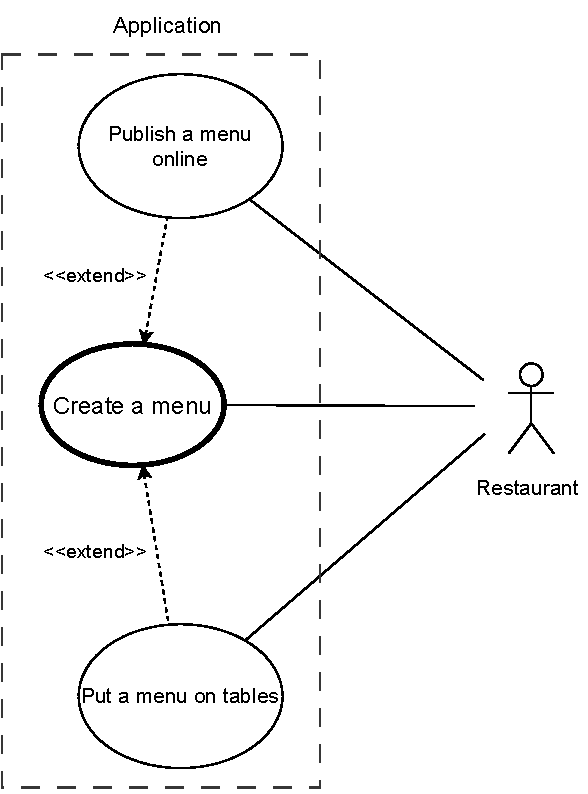
\includegraphics[width=0.62\linewidth]{master-thesis/img/use_cases/use_cases_restaurant_publish_menu}
  \caption{Restaurant offer use cases}
\end{figure}

\begin{figure}[h]
  \centering
  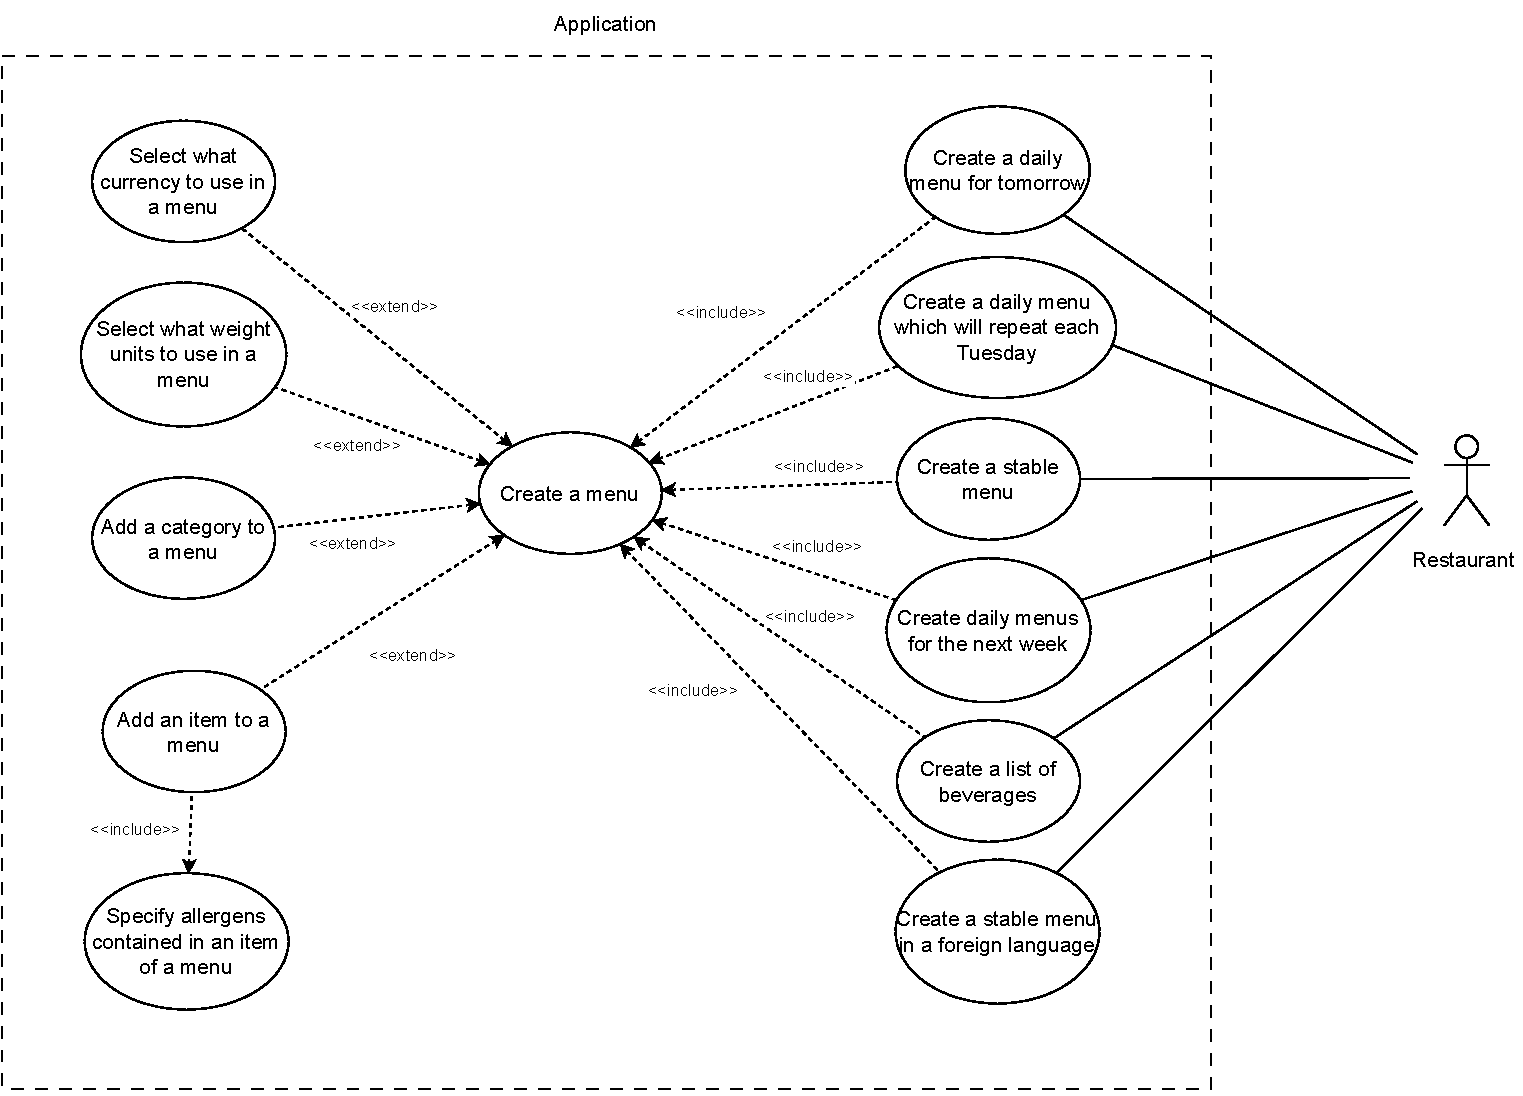
\includegraphics[width=0.62\linewidth]{master-thesis/img/use_cases/use_cases_restaurant_create_menu}
  \caption{Restaurant menu creation use cases}
\end{figure}

\begin{figure}[h]
  \centering
  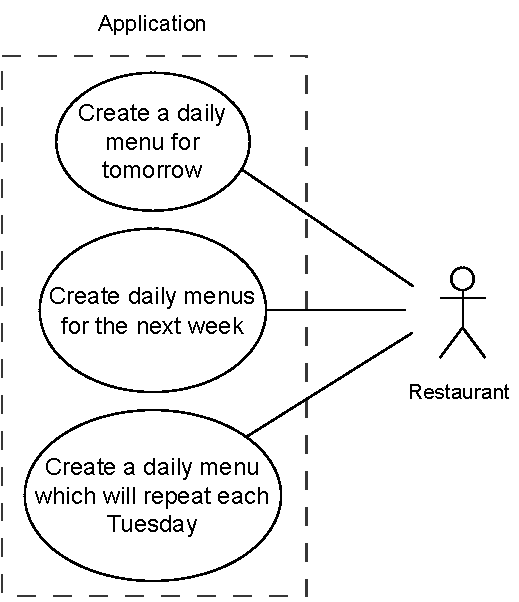
\includegraphics[width=0.62\linewidth]{master-thesis/img/use_cases/use_cases_restaurant_create_daily_menu}
  \caption{Restaurant daily menu creation use cases}
\end{figure}



% \noindent \textbf{9. Use case: Allow my guests to view a menu by scanning a QR code}

% \begin{center}
%   \begin{tabular}{| l | p{10.75cm} |}
%     \hline
%     Actor        & Restaurant \\
%     \hline
%     Description  & A restaurant's management would like to provide a menu with a QR code which will take the restaurant's guests to the application. \\
%     \hline
%     Scenario     &
%     \begin{minipage}[t]{\linewidth}
%       \begin{enumerate}[leftmargin=*,nosep,before=\vspace{-0.575\baselineskip},after=\strut]
%         \item The restaurant employee creates a menu as in use case x, ensuring that a checkbox labeled "Add a QR code" is checked. \textbf{A1}
%         \item The application generates a QR code which will link a guest to the application.
%         \item The restaurant employee prints the menu and puts in on tables as in use case x.
%         \item A guest scans the QR code on the printed menu.
%         \item The application displays the menu.
%       \end{enumerate}
%     \end{minipage}
%     \\
%     \hline
%     Alternatives &
%     \begin{minipage}[t]{\linewidth}
%       \begin{description}[nosep,after=\strut]
%         \item [A1:] The restaurant employee selects a menu from previously created menus.
%       \end{description}
%     \end{minipage}
%     \\
%     \hline
%   \end{tabular}
%   \newline
% \end{center}

% \noindent \textbf{13. Use case: Reuse an existing daily menu for today.}

% \begin{center}
%   \begin{tabular}{| l | p{10.75cm} | }
%     \hline
%     Actor        & Restaurant \\
%     \hline
%     Description  &  \\
%     \hline
%     Scenario     &
%     \begin{minipage}[t]{\linewidth}
%       \begin{enumerate}[leftmargin=*,nosep,before=\vspace{-0.575\baselineskip},after=\strut]
%         \item The restaurant employee logs in to the application.
%         \item The restaurant employee clicks a button labeled "Create new menu". \textbf{A1}
%         \item The application asks the restaurant employee what kind of menu they would like to create.
%         \item The restaurant employee selects that they wish to create a daily menu.
%         \item The application asks the restaurant employee whether they want to use an existing menu as a template.
%         \item The restaurant employee confirms by clicking a "Yes" button.
%         \item The application displays a list of menus as possible templates.
%         \item The restaurant employee chooses a menu from the list.
%         \item The application loads the chosen menu.
%         \item The restaurant employee changes the date of validity of the menu.
%         \item The restaurant employee clicks a "Save menu" button.
%         \item The application asks the restaurant employee whether they would like to overwrite the existing menu.
%         \item The restaurant employee denies by clicking a "No, create a new menu" button. \textbf{A2}
%         \item The application saves the menu.
%       \end{enumerate}
%     \end{minipage}
%     \\
%     \hline
%     Alternatives &
%     \begin{minipage}[t]{\linewidth}
%       \begin{description}[nosep,after=\strut]
%         \item [A1:] The restaurant employee clicks an "Edit" button next to a menu which they want to reuse. The restaurant employee edits a date field which controls for which day the menu is valid. The restaurant employee then clicks a "Save menu" button and the application saves the menu.
%         \item [A2:] The restaurant employee confirms by clicking a "Yes" button and the application overwrites the old menu with the new one.
%       \end{description}
%     \end{minipage}
%     \\
%     \hline
%   \end{tabular}
%   \newline
% \end{center}

